\documentclass[conference,a4paper]{IEEEtran}
\usepackage{cite,amsmath,graphicx,booktabs,url,array,tikz,pgfplots}
\usetikzlibrary{positioning,arrows.meta,patterns}
\pgfplotsset{compat=1.16, width=\columnwidth, height=4.9cm, ymin=0, ymax=105, ymajorgrids, grid style={gray!30}, tick label style={font=\footnotesize}, label style={font=\footnotesize}, legend style={font=\scriptsize, draw=none, at={(0.5,1.02)}, anchor=south, legend columns=-1, /tikz/every even column/.append style={column sep=4pt}}}
\pgfplotscreateplotcyclelist{kioskbars}{{fill=gray!20,draw=black},{fill=gray!55,draw=black},{fill=black!85,draw=black}}
\pgfplotscreateplotcyclelist{kioskpair}{{fill=gray!25,draw=black},{fill=black!80,draw=black}}
\newcommand{\figwidth}{0.98\columnwidth}

\begin{document}

\title{Consent-Based Smart Receptionist Kiosk: Face Check-In with From-Scratch Eigenfaces, Homomorphic Light Correction, and Dual-Feature Liveness}

\author{\IEEEauthorblockN{Abdulrahman Alsheikh, Fahad Al-Thani, Hadi Sleiman,\\ Islam Alshiss, Hashir Khan}
\IEEEauthorblockA{Department of Computer Science and Engineering, Qatar University, Doha, Qatar\\ CMAI 480 Computer Vision, Fall 2026}}

\maketitle

\begin{abstract}
Checking visitors in by hand is slow, repetitive, and makes people say their names aloud in a waiting room. We present a consent-based kiosk that uses a visitor's face only after the visitor agrees, and that offers an equal booking-code path to anyone who declines or cannot be recognized. Written entirely in GNU Octave, the system finds the face with a template of gradient orientation histograms slid over an image pyramid, corrects the lighting with a homomorphic filter, checks liveness with Local Binary Pattern texture and an eye-blink cue, and recognizes the visitor with Eigenfaces that we implemented from the equations, comparing only with the people booked that day. A ready-made VGG-Face model serves strictly as a competitor. On 3,764 public face images and 50 public videos, face localization reaches 99.7\% at an overlap of 0.5. Eigenfaces reach 78.1\% top-1 accuracy for a 5-person list and 45.8\% for 50 people, against 99.7\% and 99.5\% for VGG-Face. Homomorphic filtering raises Eigenfaces accuracy under harsh light from 23.9\% to 77.9\%. Dual-feature liveness passes 80\% of real clips and stops every printed-photo clip, while replay from screens remains the hardest attack.
\end{abstract}

\begin{IEEEkeywords}
face recognition, Eigenfaces, liveness detection, homomorphic filtering, local binary patterns, consent, GNU Octave
\end{IEEEkeywords}

\section{Introduction}
We present a kiosk that lets a visitor with an appointment check in without waiting for the receptionist, and that uses the visitor's face only with permission. The kiosk finds the face, confirms that it belongs to a live person, and compares it only with the people expected that day. Our main result is a measured comparison between a small system built from course methods and a state-of-the-art model, which shows where the simple method is sufficient and where it is not.

\subsection{Statement of the Problem}
A visitor must be matched to the day's list quickly and privately. The system must not be fooled by a photo or a screen, must keep working under changing office light, and must never be the only way in, since some visitors wear face coverings and some simply refuse.

\subsection{Motivation}
Today the receptionist checks each name by hand, one person at a time. This is slow when several visitors arrive together, it is the same job repeated all day, and the visitor must say a name aloud in a full waiting room. Because each day's list is short, usually 10 to 50 people, our research question is whether a method simple enough to write from the equations is sufficient for this task.

\subsection{Problem Solution}
The screen first asks for consent, and the camera stays off until the visitor agrees. The kiosk then records three seconds of video, locates the face, runs two liveness checks, corrects the lighting, and matches the face against today's list. A visitor who declines, or who fails any step, uses a booking code on the same screen, and the receptionist's list updates either way.

\subsection{Results and Conclusions}
Eigenfaces work moderately well on short lists (78.1\% for 5 people) and degrade to 45.8\% for 50 people on a hard multi-session dataset, while the ready-made model stays near 99.5\%. The homomorphic filter recommended by our instructor is effective under harsh light. Liveness stops printed photos but not screens reliably. We therefore conclude that simple methods are viable only for very short lists in controlled light, and that the booking-code path is essential rather than optional.

\subsection{Contributions, Scope, and Ethics}
Our contributions are (1) a complete kiosk in Octave built from course methods, with the face finder, Eigenfaces, the homomorphic filter, Local Binary Patterns (LBP), and the blink cue written from first principles; (2) a graph of accuracy as the daily list grows from 5 to 50 people; (3) a per-attack liveness report rather than a single average; and (4) a failure analysis under head turn, glasses, a mask, and backlight. Our success criteria are measurable: accuracy against list size, attack pass rate for each attack, check-in time for each path, and the conditions that break the system. We handle one visitor at a time, with no cloud service, booking-system link, or door control. Ethically, face data is sensitive: the kiosk asks first, keeps the camera off until consent, compares a face only with photographs of the people expected that day, keeps no picture after check-in, and always offers a non-biometric path. All evaluation data comes from public research datasets.

\section{Related Work}
\emph{Face detection.} Viola and Jones introduced cascades of simple features for real-time detection~\cite{viola}. Region-based networks later replaced hand-crafted features, and YOLO reduced detection to one forward pass~\cite{yolo}. Fully convolutional networks showed that a classifier can output a spatial map rather than one label~\cite{fcn}. Current practice is represented by Ultralytics YOLO26, an end-to-end model that removes non-maximum suppression~\cite{ultralytics}, and by NVIDIA DeepStream pipelines that pair periodic detection with a tracker~\cite{deepstream}. These tools depend on Python or GPU toolchains that fall outside our Octave environment, and our instructor allowed a ready-made model only as a competitor to our own method. We therefore locate the face with gradient orientation histograms, in the spirit of the SIFT descriptor~\cite{sift} and histograms of oriented gradients~\cite{hog}.

\emph{Face recognition.} Eigenfaces~\cite{turk} represent a face by its projection on the principal components of a training set, and are known to be sensitive to lighting and pose; Fisherfaces~\cite{fisher} address part of this. Deep embeddings such as VGG-Face~\cite{vggface}, FaceNet~\cite{facenet}, and ArcFace~\cite{arcface} define the current state of the art and motivate our choice of a ready-made competitor.

\emph{Illumination.} Homomorphic filtering~\cite{oppenheim} separates slowly varying illumination from reflectance in the log domain. Tan and Triggs~\cite{tan} later showed the value of such preprocessing for face recognition under difficult lighting, and the Yale B database~\cite{yaleb} became the standard test.

\emph{Liveness.} Texture methods based on LBP~\cite{ojala} detect the micro-texture of printed and displayed faces~\cite{maatta,chingovska}. Physical cues include eye blinks, measured from image sequences~\cite{pan} or facial landmarks~\cite{ear}. Large benchmarks such as CelebA-Spoof~\cite{celebaspoof} show that no single cue suffices, which supports the dual-feature design requested by our instructor.

\section{Proposed System}
Fig.~\ref{fig:system} shows the design. Every step uses material from the course, as listed in Table~\ref{tab:sources}.

\begin{figure}[t]
\centering
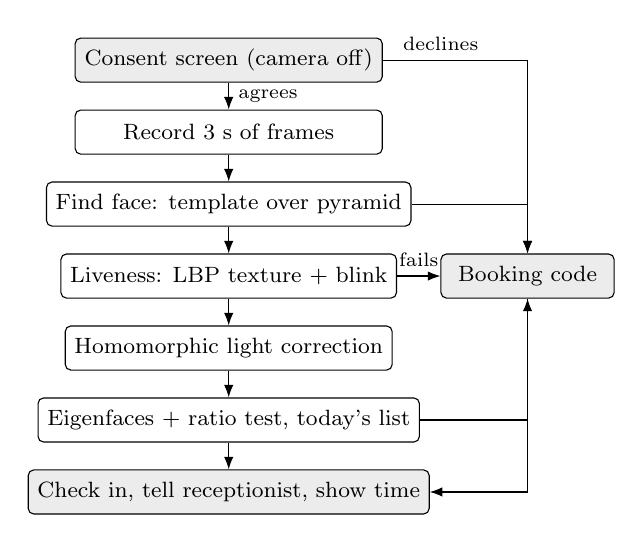
\begin{tikzpicture}[node distance=0.34cm, box/.style={draw, rounded corners=2pt, minimum width=3.9cm, minimum height=0.56cm, font=\footnotesize, align=center}, side/.style={draw, rounded corners=2pt, minimum width=2.2cm, minimum height=0.56cm, font=\footnotesize, align=center, fill=gray!15}, arr/.style={-{Latex[length=1.6mm]}, thin}]
\node[box, fill=gray!15] (c) {Consent screen (camera off)};
\node[box, below=of c] (r) {Record 3 s of frames};
\node[box, below=of r] (f) {Find face: template over pyramid};
\node[box, below=of f] (l) {Liveness: LBP texture + blink};
\node[box, below=of l] (h) {Homomorphic light correction};
\node[box, below=of h] (e) {Eigenfaces + ratio test, today's list};
\node[box, below=of e, fill=gray!15] (d) {Check in, tell receptionist, show time};
\node[side, right=0.55cm of l] (b) {Booking code};
\draw[arr] (c) -- node[right, font=\scriptsize] {agrees} (r);
\draw[arr] (r) -- (f);
\draw[arr] (f) -- (l);
\draw[arr] (l) -- (h);
\draw[arr] (h) -- (e);
\draw[arr] (e) -- (d);
\draw[arr] (c.east) -| node[pos=0.2, above, font=\scriptsize] {declines} (b.north);
\draw[arr] (f.east) -| (b.north);
\draw[arr] (l.east) -- node[above, font=\scriptsize] {fails} (b.west);
\draw[arr] (e.east) -| (b.south);
\draw[arr] (b.south) |- (d.east);
\end{tikzpicture}
\caption{High-level design of the kiosk. A visitor who declines or fails any step uses the booking code.}
\label{fig:system}
\end{figure}

\begin{table}[t]
\caption{Where each step comes from in the course}
\label{tab:sources}
\centering\footnotesize
\begin{tabular}{@{}p{2.6cm}p{5.3cm}@{}}
\toprule
Step & Course source \\
\midrule
Camera capture & Assignment 2, Question 1 \\
Face localization & Assignment 2 (gradient orientation); Feature Extraction Part 2 (cell histograms, image pyramids) and Part 3 (correlation); Lecture 8 (sliding window) \\
Light correction & Ch.~3 (illumination shading, Gaussian filter); instructor's comment \\
Eigenfaces & Ch.~2 Linear Algebra (eigenspace for face recognition); Assignment 1 (\texttt{eig} of $A^TA$) \\
Matching and ratio & Feature Extraction Part 3 (Euclidean distance); Assignment 3 (ratio test) \\
LBP texture & Ch.~3 ($N_8$ neighbors); Assignment 2 (histograms); instructor's comment \\
Blink cue & Feature Extraction Part 3 (NCC); instructor's comment \\
Competitor model & Lecture 5 (VGG-16, global average pooling), Lecture 6 (transfer learning) \\
Metrics & Lecture 3 (precision, recall, F1), Lecture 8 (IoU) \\
\bottomrule
\end{tabular}
\end{table}

\subsection{Face Localization}
We compute the image gradient and, as in the SIFT descriptor, an 8-bin histogram of gradient orientation in every cell of $8\times8$ pixels. Each cell is normalized, so that lighting has little effect. The face template is the average of these cell histograms over 150 labeled training faces and their mirror images, stored as $12\times8$ cells, with the mean of each bin subtracted. We slide the template over ten levels of an image pyramid with scale ratio 1.15, which covers face heights from 127 to 445 pixels, by correlating it with the cell histograms. The strongest match is taken as the face, and a match below a fixed value means that nobody is in front of the camera. The visitor stands still during the three seconds, so the same box is used in every frame.

\subsection{Homomorphic Light Correction}
An image is modeled as illumination times reflectance, $I = L \cdot R$. The logarithm turns the product into a sum, and slow changes in the log image are mostly illumination. With a Gaussian low-pass filter $G_\sigma$ we compute
\begin{equation}
O = \gamma_L \, (G_\sigma * \log I) + \gamma_H \, (\log I - G_\sigma * \log I),
\end{equation}
with $\sigma=8$, $\gamma_L=0.7$, $\gamma_H=1.4$. Because the course covers filtering in the spatial domain, we apply the Gaussian with \texttt{imgaussfilt} rather than in the frequency domain. The result is normalized to zero mean and unit variance. We selected these values on Yale people 1--19 and report results on people 20--38.

\subsection{Eigenfaces from the Equations}
Each enrolled face is resized to $80\times60$ pixels and stacked as a column. With $A$ holding the mean-subtracted faces, we compute the eigenvectors $v$ of the small matrix $A^TA$ and obtain the eigenfaces as normalized columns of $U = Av$, following the relation between $A^TA$ and $AA^T$ from our linear algebra review. A face is described by its weights $w = U^T(x - \bar{x})$. The visitor is the nearest enrolled face by Euclidean distance. To reject strangers we use the ratio test from feature matching: the match is accepted only if the distance to the nearest person, divided by the distance to the next different person, is below 0.85.

\subsection{Dual-Feature Liveness}
\emph{Texture.} LBP compares each pixel with its eight neighbors and forms an 8-bit code. The 256-bin histogram of codes, averaged over the frames of the face, describes micro-texture. A face passes when its histogram is closer to the mean histogram of real faces than to that of fake faces.

\emph{Blink.} A blink changes the eyes while the lower face stays the same. In each frame we compute the correlation of the eye band and of the lower-face band with their median appearance. The blink score is the largest amount by which the lower face stayed similar while the eyes did not. The kiosk requires both checks to pass.

\subsection{Ready-Made Competitor}
As a competitor only, we run the pretrained convolution layers of VGG-16~\cite{vgg} trained on faces~\cite{vggface} on a $224\times224$ crop and apply global average pooling, which yields a 512-value embedding compared by Euclidean distance. This model appears only in our experiments, on the same detected face crops as Eigenfaces, and never runs in the kiosk.

\subsection{Kiosk Application}
Fig.~\ref{fig:gui} shows the screen, built with Octave graphical controls. It holds the consent notice, both check-in paths, and the receptionist's list. Error cases, such as a missing camera, an unknown code, an empty field, or repeated clicks, produce a message rather than a crash. The receptionist's list shows how each visitor checked in and, for a face check-in, how long it took. Today's list is a folder of photographs of the visitors expected that day, one subfolder per visitor, named with the visitor and the booking code.

\begin{figure}[t]
\centering
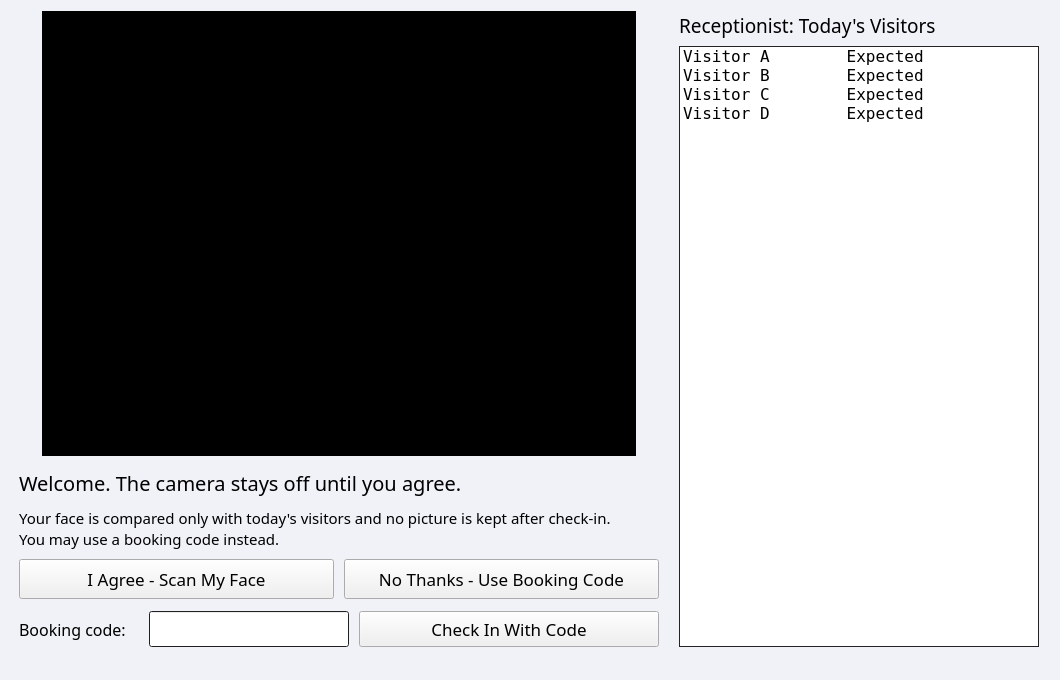
\includegraphics[width=\figwidth]{kiosk_screen.png}
\caption{The kiosk screen: camera view and consent (left), receptionist's list (right).}
\label{fig:gui}
\end{figure}

\section{Experimental Results}

\subsection{Data and Setup}
Table~\ref{tab:data} lists the public datasets, which replace the team's own faces planned in our proposal. All programs ran in GNU Octave 11.1 on a laptop CPU (Intel Core i5-1038NG7, 4 cores, 16~GB RAM). Unless stated otherwise, Eigenfaces include the homomorphic filter, each person is enrolled with 5 images, and results use the detected face box, so errors in face localization are included. All random choices use fixed seeds, and the list-size and glasses tests are repeated over 20 random lists.

\begin{table}[t]
\caption{Public data used}
\label{tab:data}
\centering\footnotesize
\begin{tabular}{@{}>{\raggedright\arraybackslash}p{2.25cm}>{\raggedright\arraybackslash}p{1.75cm}>{\raggedright\arraybackslash}p{3.75cm}@{}}
\toprule
Dataset & Size & Use \\
\midrule
Georgia Tech~\cite{gatech} & 50 people, 750 images & Face boxes, list size, strangers, glasses, mask, backlight \\
FEI part 1~\cite{fei} & 50 people, 600 images used & Head turn \\
Cropped Yale B~\cite{yaleb} & 38 people, 2,414 images & Changing light \\
Web-camera clips~\cite{unique} & 40 videos & Real, print, cut print, monitor \\
Phone replay~\cite{axon} & 10 videos & Phone-screen attack \\
\bottomrule
\end{tabular}
\end{table}

\subsection{Face Localization}
The template was learned from 150 Georgia Tech images. On the other 600 images of the same 50 people, the box overlaps the labeled face with an intersection over union (IoU) of at least 0.5 in 99.7\% of cases, with a mean IoU of 0.82 and 0.21~s per frame. On webcam clips of real people, which have no labels, visual inspection of the 28 middle frames found the box on the face in 26; one frame reported no face and one box was wrong.

\subsection{Accuracy as the List Grows}
Fig.~\ref{fig:list} and Table~\ref{tab:list} answer the central question of our proposal. Eigenfaces fall from 78.1\% at 5 people to 45.8\% at 50 people, because each new person adds another nearby candidate. VGG-Face remains at 99.5\% or above.

\begin{figure}[t]
\centering
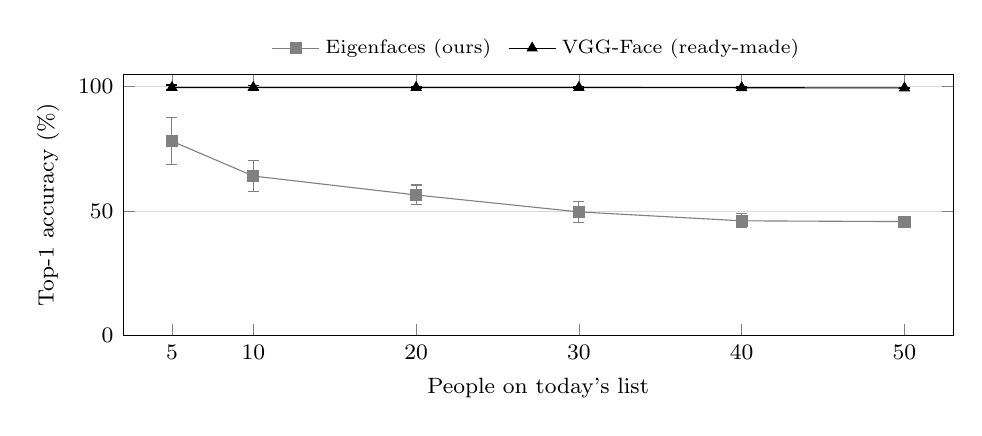
\begin{tikzpicture}
\begin{axis}[xlabel={People on today's list}, ylabel={Top-1 accuracy (\%)}, xtick={5,10,20,30,40,50}, xmin=2, xmax=53, error bars/y dir=both, error bars/y explicit]
\addplot[gray, mark=square*] coordinates {(5,78.1) +- (0,9.5) (10,64.1) +- (0,6.3) (20,56.5) +- (0,4.0) (30,49.7) +- (0,4.3) (40,46.1) +- (0,2.8) (50,45.8) +- (0,1.7)};
\addplot[black, mark=triangle*] coordinates {(5,99.7) +- (0,1.0) (10,99.7) +- (0,0.8) (20,99.7) +- (0,0.5) (30,99.7) +- (0,0.3) (40,99.6) +- (0,0.3) (50,99.5) +- (0,0.2)};
\legend{Eigenfaces (ours), VGG-Face (ready-made)}
\end{axis}
\end{tikzpicture}
\caption{Top-1 accuracy as today's list grows, mean and standard deviation over 20 random lists.}
\label{fig:list}
\end{figure}

\begin{table}[t]
\caption{Top-1 accuracy (\%) against list size}
\label{tab:list}
\centering\footnotesize
\begin{tabular}{@{}lrrrrrr@{}}
\toprule
People on list & 5 & 10 & 20 & 30 & 40 & 50 \\
\midrule
Eigenfaces & 78.1 & 64.1 & 56.5 & 49.7 & 46.1 & 45.8 \\
VGG-Face & 99.7 & 99.7 & 99.7 & 99.7 & 99.6 & 99.5 \\
\bottomrule
\end{tabular}
\end{table}

\subsection{Visitors Versus Strangers}
A kiosk must also reject people who are not on the list. We enrolled 25 people and tested with them and with 25 unknown people. At the kiosk's ratio limit, Eigenfaces reach precision 0.79, recall 0.36, and F1 0.49, and accept 5.3\% of strangers, because the correct person is often not the nearest match. VGG-Face reaches 0.96, 0.98, and 0.97, accepting 2.4\%. We keep the strict limit deliberately, since a rejected visitor can use the booking code.

\subsection{Changing Light}
Fig.~\ref{fig:light} tests the instructor's suggestion on unseen Yale people, enrolled under near-frontal light. Under moderate side light, accuracy is 88.2\% without correction and 98.4\% with the homomorphic filter. Under harsh light, it rises from 23.9\% to 77.9\%. This is the clearest gain in the project.

\begin{figure}[t]
\centering
\begin{tikzpicture}
\begin{axis}[ybar, bar width=20pt, cycle list name=kioskpair, ymax=118, ylabel={Top-1 accuracy (\%)}, symbolic x coords={Moderate side light, Harsh side light}, xtick=data, enlarge x limits=0.45, nodes near coords, every node near coord/.append style={font=\tiny}]
\addplot coordinates {(Moderate side light,88.2) (Harsh side light,23.9)};
\addplot coordinates {(Moderate side light,98.4) (Harsh side light,77.9)};
\legend{No correction, Homomorphic filter}
\end{axis}
\end{tikzpicture}
\caption{Eigenfaces under changing light on people not used for tuning.}
\label{fig:light}
\end{figure}

\subsection{Liveness per Attack}
Table~\ref{tab:live} and Fig.~\ref{fig:live} report pass rates per clip. A clip passes if any of up to four 3-second windows passes, which matches a visitor being allowed to retry. Texture models were trained on half of the clips and tested on the other half. Combining both cues stops every printed-photo clip and 100\% of cut-print clips, and lets 80\% of real clips through. Screens are the hardest attacks: 70\% of laptop-monitor clips and 50\% of phone clips pass. The blink cue alone passes most attacks, because a hand-held page moves and a replayed video contains real blinks, so texture does most of the work. These figures come from only 10 clips per class and should be read as indicative.

\begin{table}[t]
\caption{Liveness pass rate per clip (\%)}
\label{tab:live}
\centering\footnotesize
\begin{tabular}{@{}lrrr@{}}
\toprule
Input & Texture & Blink & Both \\
\midrule
Real face & 80 & 90 & 80 \\
Printed photo & 0 & 100 & 0 \\
Cut print & 0 & 100 & 0 \\
Laptop monitor & 70 & 100 & 70 \\
Phone screen & 60 & 80 & 50 \\
\bottomrule
\end{tabular}
\end{table}

\begin{figure}[t]
\centering
\begin{tikzpicture}
\begin{axis}[ybar, bar width=6pt, cycle list name=kioskbars, ylabel={Clips passed (\%)}, symbolic x coords={Real, Print, Cut print, Monitor, Phone}, xtick=data, enlarge x limits=0.12]
\addplot coordinates {(Real,80) (Print,0) (Cut print,0) (Monitor,70) (Phone,60)};
\addplot coordinates {(Real,90) (Print,100) (Cut print,100) (Monitor,100) (Phone,80)};
\addplot coordinates {(Real,80) (Print,0) (Cut print,0) (Monitor,70) (Phone,50)};
\legend{Texture only, Blink only, Both (kiosk rule)}
\end{axis}
\end{tikzpicture}
\caption{Pass rate of real clips (should be high) and attacks (should be low).}
\label{fig:live}
\end{figure}

\subsection{Latency and Speed}
Table~\ref{tab:speed} lists the processing time of each step for one check-in on the CPU. Finding the face dominates the processing. Opening the camera, recording 45 frames, and showing them on the screen took 4.71~s in our measurement, longer than the nominal 3~s of video, so a face check-in takes about 5.1~s from consent to result. The booking-code lookup itself takes 0.029~ms; a visitor typing a four-digit code and pressing a button needs a few seconds more, which we estimate at about 3~s but did not measure on real users. Side by side, the booking-code path is therefore no slower than the face path, which supports treating it as an equal way in. The receptionist's list shows the measured time of every face check-in. Training Eigenfaces for a full list of 50 people takes 0.037~s once, and matching time remains negligible at every list size.

\begin{table}[t]
\caption{Processing time for one face check-in}
\label{tab:speed}
\centering\footnotesize
\begin{tabular}{@{}lr@{}}
\toprule
Step & Seconds \\
\midrule
Find face (template over pyramid) & 0.206 \\
Crop all 45 frames & 0.134 \\
LBP texture & 0.037 \\
Blink & 0.016 \\
Homomorphic filter & 0.005 \\
Match against 250 enrolled faces & 0.000 \\
\midrule
Total processing & 0.40 \\
Open camera, record and show 45 frames & 4.71 \\
\midrule
Face check-in, total & 5.1 \\
\midrule
Booking-code lookup (ms) & 0.029 \\
Train Eigenfaces, 50 people (once per list) & 0.037 \\
\bottomrule
\end{tabular}
\end{table}

\subsection{Failure Cases}
Table~\ref{tab:fail} summarizes the conditions listed in our proposal. Head turn was measured on FEI at five levels, from a small turn to full profile (Fig.~\ref{fig:turn}). Eigenfaces fall quickly as the head turns, from 50\% to 3\%, while VGG-Face stays at 91\% until nearly profile (47\% at full profile). Glasses did not hurt: the 13 people who wear glasses in some images scored 53\% against 43\% for the others, probably because the glasses themselves are distinctive. The mask and backlight were simulated on whole frames, by covering the lower 45\% of the face and by strong darkening. A mask defeats Eigenfaces (13\%), since half of the vector changes, and also harms VGG-Face (82\%). Backlight lowers Eigenfaces to 45\% against 100\% for VGG-Face. These simulated cases are approximations of real conditions. Other failures we observed include heads that are turned or bowed, tilted hand-held paper, and very close phone screens, where the template does not match the whole face.

\begin{table}[t]
\caption{Failure analysis: top-1 accuracy (\%)}
\label{tab:fail}
\centering\footnotesize
\begin{tabular}{@{}lrr@{}}
\toprule
Condition & Eigenfaces & VGG-Face \\
\midrule
Head turn, level 1 (small) & 50 & 100 \\
Head turn, level 3 & 18 & 94 \\
Head turn, level 5 (profile) & 3 & 47 \\
People who wear glasses & 53 & 99 \\
Others & 43 & 100 \\
Mask (simulated) & 13 & 82 \\
Strong backlight (simulated) & 45 & 100 \\
\bottomrule
\end{tabular}
\end{table}

\begin{figure}[t]
\centering
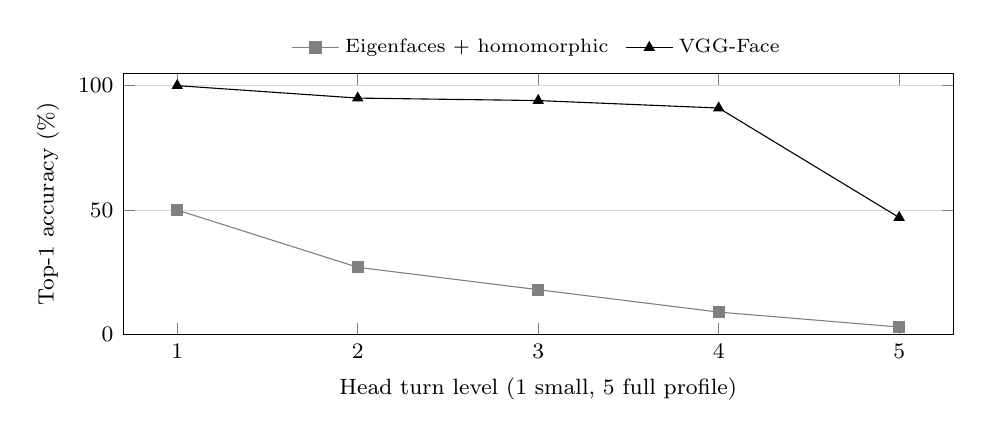
\begin{tikzpicture}
\begin{axis}[xlabel={Head turn level (1 small, 5 full profile)}, ylabel={Top-1 accuracy (\%)}, xtick={1,2,3,4,5}, xmin=0.7, xmax=5.3]
\addplot[gray, mark=square*] coordinates {(1,50.0) (2,27.0) (3,18.0) (4,9.0) (5,3.0)};
\addplot[black, mark=triangle*] coordinates {(1,100.0) (2,95.0) (3,94.0) (4,91.0) (5,47.0)};
\legend{Eigenfaces + homomorphic, VGG-Face}
\end{axis}
\end{tikzpicture}
\caption{Accuracy as the head turns from frontal to profile.}
\label{fig:turn}
\end{figure}

\subsection{Discussion}
The results agree on one theme: a method that can be explained on a page works within a narrow range. Eigenfaces compare whole pixel patterns, so anything that moves pixels, such as a head turn, a mask, or a different session, lowers accuracy, while the deep competitor has learned features invariant to these changes. Our proposal argued that a short daily list makes a simple method sufficient. The data support this only partly: accuracy is 78.1\% for 5 people and falls as the list grows. The instructor's two suggestions addressed real weaknesses, since the homomorphic filter recovers harsh lighting and texture stops printed attacks. The remaining weakness is replay from screens, and this argues for the booking-code path being equal rather than a backup.

\section{Conclusions and Future Directions}
We built a complete consent-based check-in kiosk in Octave using course methods, and we measured it honestly against a ready-made model. Eigenfaces with homomorphic filtering are usable only for very short lists in controlled conditions, face localization by matching gradient histograms is reliable, and liveness is effective against print but not yet against screens. The main limitations are the small size of the liveness set, the absence of the team's own faces, and simulated mask and backlight conditions. Future work should collect a consented local dataset, add moiré analysis for screen replay, and, if permitted, let the deep model make the identity decision, since our results show that it would serve visitors far better.

\section{Meta-Discussion}
The most difficult part was reliable face localization, because matching a template of raw pixels failed on real webcam frames until we matched gradient orientation histograms instead; the second was making the blink cue distinguish bending paper from real eyes, which remains imperfect. The least difficult parts were Eigenfaces, which follow directly from the equations, and the booking-code path.

Our implementation differs from the proposal in the following ways. We used GNU Octave rather than MATLAB, so the screen uses Octave's graphical controls in place of App Designer, and the ready-made model runs through our own forward pass in place of the Deep Learning Toolbox. We evaluated on public datasets instead of our own faces and fake samples. Face alignment is limited to locating and cropping the face.

\section*{AI Use Disclosure}
Generative AI (Claude, by Anthropic) was used to write the source code, run the experiments, and draft this report. We declare this use in accordance with the course policy on generative AI.

\begin{thebibliography}{99}
\bibitem{viola} P. Viola and M. Jones, ``Rapid object detection using a boosted cascade of simple features,'' in \emph{Proc. IEEE CVPR}, 2001, pp. 511--518.
\bibitem{yolo} J. Redmon, S. Divvala, R. Girshick, and A. Farhadi, ``You only look once: Unified, real-time object detection,'' in \emph{Proc. IEEE CVPR}, 2016, pp. 779--788.
\bibitem{fcn} J. Long, E. Shelhamer, and T. Darrell, ``Fully convolutional networks for semantic segmentation,'' in \emph{Proc. IEEE CVPR}, 2015, pp. 3431--3440.
\bibitem{ultralytics} Ultralytics, ``YOLO documentation.'' [Online]. Available: \url{https://docs.ultralytics.com/}
\bibitem{deepstream} NVIDIA, ``DeepStream SDK developer guide.'' [Online]. Available: \url{https://docs.nvidia.com/metropolis/deepstream/dev-guide/}
\bibitem{sift} D. G. Lowe, ``Distinctive image features from scale-invariant keypoints,'' \emph{Int. J. Comput. Vis.}, vol. 60, no. 2, pp. 91--110, 2004.
\bibitem{hog} N. Dalal and B. Triggs, ``Histograms of oriented gradients for human detection,'' in \emph{Proc. IEEE CVPR}, 2005, pp. 886--893.
\bibitem{turk} M. Turk and A. Pentland, ``Eigenfaces for recognition,'' \emph{J. Cogn. Neurosci.}, vol. 3, no. 1, pp. 71--86, 1991.
\bibitem{fisher} P. N. Belhumeur, J. P. Hespanha, and D. J. Kriegman, ``Eigenfaces vs. Fisherfaces: Recognition using class specific linear projection,'' \emph{IEEE Trans. Pattern Anal. Mach. Intell.}, vol. 19, no. 7, pp. 711--720, Jul. 1997.
\bibitem{vggface} O. M. Parkhi, A. Vedaldi, and A. Zisserman, ``Deep face recognition,'' in \emph{Proc. BMVC}, 2015.
\bibitem{facenet} F. Schroff, D. Kalenichenko, and J. Philbin, ``FaceNet: A unified embedding for face recognition and clustering,'' in \emph{Proc. IEEE CVPR}, 2015, pp. 815--823.
\bibitem{arcface} J. Deng, J. Guo, N. Xue, and S. Zafeiriou, ``ArcFace: Additive angular margin loss for deep face recognition,'' in \emph{Proc. IEEE/CVF CVPR}, 2019, pp. 4690--4699.
\bibitem{oppenheim} A. V. Oppenheim, R. W. Schafer, and T. G. Stockham, ``Nonlinear filtering of multiplied and convolved signals,'' \emph{Proc. IEEE}, vol. 56, no. 8, pp. 1264--1291, Aug. 1968.
\bibitem{tan} X. Tan and B. Triggs, ``Enhanced local texture feature sets for face recognition under difficult lighting conditions,'' \emph{IEEE Trans. Image Process.}, vol. 19, no. 6, pp. 1635--1650, Jun. 2010.
\bibitem{yaleb} A. S. Georghiades, P. N. Belhumeur, and D. J. Kriegman, ``From few to many: Illumination cone models for face recognition under variable lighting and pose,'' \emph{IEEE Trans. Pattern Anal. Mach. Intell.}, vol. 23, no. 6, pp. 643--660, Jun. 2001.
\bibitem{ojala} T. Ojala, M. Pietik\"ainen, and T. M\"aenp\"a\"a, ``Multiresolution gray-scale and rotation invariant texture classification with local binary patterns,'' \emph{IEEE Trans. Pattern Anal. Mach. Intell.}, vol. 24, no. 7, pp. 971--987, Jul. 2002.
\bibitem{maatta} J. M\"a\"att\"a, A. Hadid, and M. Pietik\"ainen, ``Face spoofing detection from single images using micro-texture analysis,'' in \emph{Proc. IJCB}, 2011, pp. 1--7.
\bibitem{chingovska} I. Chingovska, A. Anjos, and S. Marcel, ``On the effectiveness of local binary patterns in face anti-spoofing,'' in \emph{Proc. BIOSIG}, 2012, pp. 1--7.
\bibitem{pan} G. Pan, L. Sun, Z. Wu, and S. Lao, ``Eyeblink-based anti-spoofing in face recognition from a generic webcamera,'' in \emph{Proc. IEEE ICCV}, 2007, pp. 1--8.
\bibitem{ear} T. Soukupov\'a and J. \v{C}ech, ``Real-time eye blink detection using facial landmarks,'' in \emph{Proc. Comput. Vis. Winter Workshop}, 2016.
\bibitem{celebaspoof} Y. Zhang \emph{et al.}, ``CelebA-Spoof: Large-scale face anti-spoofing dataset with rich annotations,'' in \emph{Proc. ECCV}, 2020, pp. 70--85.
\bibitem{vgg} K. Simonyan and A. Zisserman, ``Very deep convolutional networks for large-scale image recognition,'' in \emph{Proc. ICLR}, 2015.
\bibitem{gatech} A. V. Nefian, ``Georgia Tech face database.'' [Online]. Available: \url{http://www.anefian.com/research/face_reco.htm}
\bibitem{fei} C. E. Thomaz and G. A. Giraldi, ``A new ranking method for principal components analysis and its application to face image analysis,'' \emph{Image Vis. Comput.}, vol. 28, no. 6, pp. 902--913, Jun. 2010.
\bibitem{unique} UniqueData, ``Web camera face liveness detection dataset.'' [Online]. Available: \url{https://huggingface.co/datasets/UniqueData/web-camera-face-liveness-detection}
\bibitem{axon} AxonData, ``Face anti-spoofing dataset.'' [Online]. Available: \url{https://huggingface.co/datasets/AxonData/face-anti-spoofing-dataset}
\end{thebibliography}

\end{document}
